\chapter{Background}
\label{ch:bg}

This chapter provides the queueing network vocabulary the rest of the report relies on. We first introduce the modelling structures and laws in Section~\ref{sec:bg-modelling}, look at how these laws can be manipulated to solve queueing network models through Mean Value Analysis (MVA) in Section~\ref{sec:bg-mva}, and then consider the modelling situations in which the assumptions break and look at the client--server extensions that motivate Layered Queueing Networks in Section~\ref{sec:bg-extended}.

\section{Queueing Network Modelling}
\label{sec:bg-modelling}

Queueing networks provide a formal abstraction for evaluating performance in computer systems, where jobs (or \textit{customers}) contend for shared system resources. These networks enable analysts to derive key metrics, such as utilisation, throughput and response time, without requiring fully built systems and intense simulation. This section introduces the structure and principles of underlying queueing models, including their components, performance laws and outputs, with a focus on separable product-form models.

\subsection{Basics}
\label{sec:bg-basics}

A queueing network model represents a system using two primary entities: \textit{customers}, which model users or transactions, and \textit{service centres}, which model resources such as CPUs, disks, or servers. These components have a close correspondence to the attributes of real computer systems, allowing them to be modelled naturally.

\subsubsection*{Customers}

The behaviour of customers can be characterised into three types, enabling the modelling of systems of various forms, as specified by the \textit{workload intensities} shown below \cite{lazowska84}:

\begin{itemize}
\item A \textbf{transaction workload} represents independent requests arriving from the outside world, behaviour typical of API calls and database queries. This arrival-driven workload is specified by the arrival rate $\lambda$ at which jobs arrive into the system. Customers are serviced and then leave the model on completion, causing a population that varies over time.
\item A \textbf{batch workload} represents a fixed number of jobs inside the system. This is typical of analytical jobs, and it works under the assumption that when a job finishes and leaves the system it is immediately replaced by another job from the same workload. This ensures a constant population size, specified by parameter $N$, relating to the average population size of the true workload.
\item A \textbf{terminal workload} models jobs that pause between requests, typical of timesharing systems and interactive users. Again, the population is fixed by parameter $N$, however instead of exiting the system and being replaced immediately, the user \textit{thinks} for a specified time $Z$ before submitting the next request.
\end{itemize}

A model that contains only transaction workloads is known as an \textbf{open model}, as there is an infinite stream of incoming transactions causing varied population size, whilst a model that contains only batch and terminal workloads is a \textbf{closed model} as it consists of a fixed number of customers that re-circulate. A model that consists of both open and closed classes is known as a mixed model \cite{lazowska84}.

For the purpose of this project, we will only consider closed models. This is a deliberate scoping decision as closed models are the standard formalism for enterprise software performance analysis since interactive users, microservice request loops and bounded job pools all naturally circulate a fixed customer population through the system rather than admitting an unbounded external stream \cite{lazowska84}.

\subsubsection*{Service Centres}

Service centres represent any system resource that provides service to customers, and can be of two different types \cite{lazowska84}:

\begin{itemize}
\item \textbf{Queueing centres} are service centres where customers compete for a limited resource. Customers may experience a \textit{wait time} whilst they are in the queue before the resource becomes available, they then spend the necessary \textit{service time} at the resource. Queueing centres are used to model computing resources such as CPU or disk. A scheduling discipline (FCFS, LCFS, SIRO, PS, IS) can also be established for models with multiple types of customers \cite{baskett75,spirn79}.
\item \textbf{Delay centres} are service centres where customers do not compete, instead treated as having their own server. This means there is no queue and therefore no wait time, just the service time specified. Delay centres can be used to model user think time or fixed communication delays.
\end{itemize}

\subsubsection*{Service Demands}

Service centres must specify the amount of time required for a customer to be served, denoted $D_k$ for service centre $k$. The service demand can be thought of as $B_k/C$, where $B_k$ is the total busy time at service centre $k$ and $C$ is the total number of system completions, or as $V_k \cdot S_k$, where $V_k$ is the number of visits made to service centre $k$ and $S_k$ is the service requirement per visit to $k$.  We let $D$ be the total service demand for customers at all centres, such that $D \equiv \sum_{k=1}^{K} D_k$ \cite{lazowska84}.

\subsubsection*{Visualising Models}

Now that we have an understanding of these models, we are able to visualise them. Figure \ref{fig:bg-computer-system-model} shows how these service centres can be combined and applied to a real computing problem. This model characterises a computer system, representing each system resource (a CPU and three disks) as separate queueing centres and representing customer arrival via a delay centre \cite{lazowska84}.

\begin{figure}[h]
  \centering
  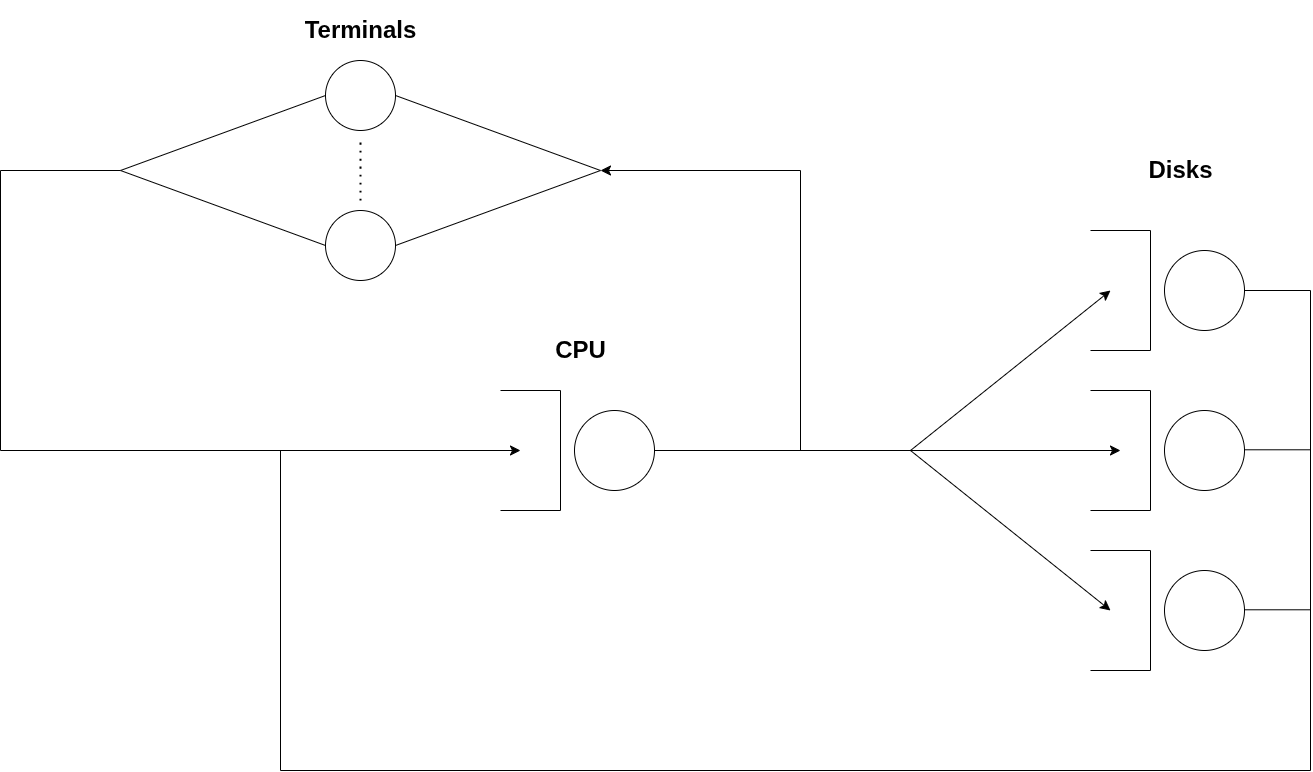
\includegraphics[width=0.5\textwidth]{figures/model2.png}
  \caption{A computer system model.}
  \label{fig:bg-computer-system-model} 
\end{figure}


\subsection{Laws}
\label{sec:bg-laws}

It is now possible to look into some of the fundamental laws of queueing network systems that will help form our analysis techniques.

\subsubsection*{Basic Quantities}

It is first worth considering the system as a whole. We can measure the \textbf{observation period} $T$, the number of \textbf{arrivals} $A$, the number of \textbf{completions} $C$, and the \textbf{busy time} $B$ for which the resource was observed to be in use. From these we can calculate the \textbf{arrival rate} $\lambda = A/T$, the \textbf{throughput} $X = C/T$, the \textbf{utilisation} $U = B/T$, and \textbf{mean service requirement} $S = B/C$ of jobs \cite{lazowska84}.

\subsubsection*{Utilisation Law}

By considering that $B/T = (C/T)(B/C)$, we can derive the utilisation law, stating that the utilisation of the system is equal to the product of the throughput and the service requirement \cite{lazowska84}:

\begin{equation}
U = X \cdot S
\label{eq:utilisation-law}
\end{equation}

\subsubsection*{Little's Law}

The most useful law we will come across is Little's Law. First we need to define a few new quantities: the \textbf{accumulated time in the system} $W$, the \textbf{average number of requests in the system} $N = W/T$, and the \textbf{average system residence time per request} $R = W/C$ \cite{lazowska84}.

We can now derive Little's Law from the fact that $W/T = (C/T)(W/C)$. This law states that the average population of the system is equal to the product of the throughput of the system and the average time a request spends in the system \cite{lazowska84}:

\begin{equation}
N = X \cdot R
\label{eq:littles-law}
\end{equation}

This law is important as it is widely applicable, requires only weak assumptions, and is valuable in checking the consistency of data measurements. It is also frequent for us to know two of the three quantities of the equation when studying computer systems, allowing us to calculate the third. Finally, Little's Law is the core part of the algorithms we discuss later on for evaluating queueing network models \cite{lazowska84}.

\subsubsection*{Little's Law application}

\begin{figure}[h]
  \centering
  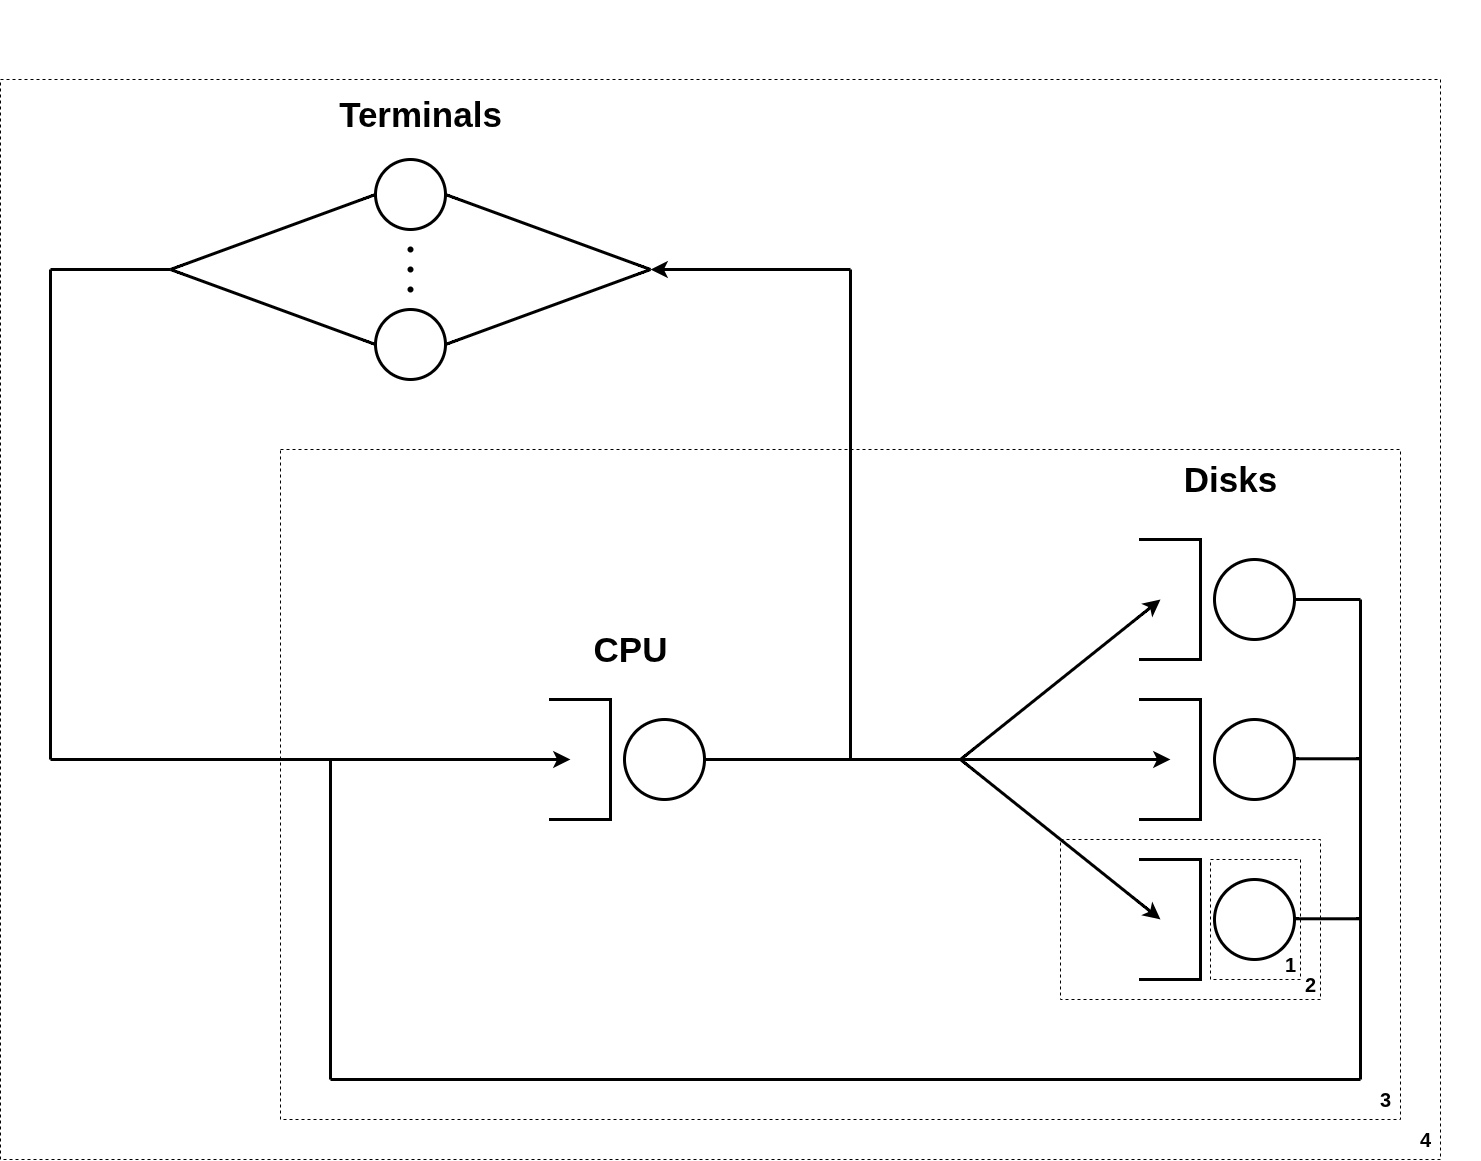
\includegraphics[width=0.6\textwidth]{figures/littles_law2.png}
  \caption{Application of Little's Law.}
  \label{fig:bg-littles-law}
\end{figure}

Figure~\ref{fig:bg-littles-law} revisits the queueing network we established earlier and lets us apply Little's Law at four levels of the system:

\begin{description}
  \item[Level 1: a single resource (server only).] Population is utilisation (0 or 1), throughput is the rate at which the resource satisfies requests, and residence time is the mean service requirement per request.
  \item[Level 2: the resource with its queue.] Population is the total number of requests in the queue or server, throughput is unchanged, and residence time is the mean time a request spends queueing and being served.
  \item[Level 3: the central subsystem.] Population is the number of customers in the central system, throughput is the rate at which interactions flow between terminals and the system, and residence time is the time between a user request and response.
  \item[Level 4: the full system, including terminals.] Population is the total number of users, throughput is unchanged, and residence time is the sum of system response time and user think time.
\end{description}


\subsubsection*{The Response Time Law}

Treating the system as a whole lets us split residence time into response time and think time, giving $N = X(R + Z)$, from which we can derive the response time law \cite{lazowska84}:

\begin{equation}
R = \frac{N}{X} - Z
\label{eq:response-time-law}
\end{equation}

\subsubsection*{The Forced Flow Law}

Another fundamental law of queueing networks states that throughput in all parts of the system must be proportional. This becomes an extremely powerful tool when combined with Little's Law. To define this we must first define the \textbf{visit count} of resource $k$ as $V_k = C_k/C$. Rearranging this as $C_k = V_k \cdot C$ and dividing through by $T$ allows us to use the definition of throughput $X = C/T$ to give us the forced flow law \cite{lazowska84}:

\begin{equation}
X_k = V_k \cdot X
\label{eq:forced-flow-law}
\end{equation}

\subsubsection*{The Flow Balance Assumption}

It may be useful to assume that the closed systems we are looking at satisfy the assumption that the number of arrivals is equal to the number of completions, $A = C$. Equivalently, the arrival rate to the system equals the throughput of the system, $\lambda = X$. This can be used in conjunction with Little's Law and the Forced Flow Law to calculate device utilisations for systems with terminal workload intensities \cite{lazowska84}.

\subsection{Outputs}
\label{sec:bg-outputs}

Once a queueing model is defined and evaluated, we are able to obtain a list of outputs useful for performance analysis. As the inputs to the model are described as averages over time, so will the outputs. We can show that the value of an output relates to a specific input through notation such as $X(N)$, where $X$ is the throughput for a batch or terminal class with population $N$. We now discuss key performance measures that will help us analyse our system \cite{lazowska84}.

\subsubsection*{Utilisation}

Denoted $U_k$, the utilisation of centre $k$ is defined as the proportion of time device $k$ is busy or, for a delay centre, the average number of customers in service there. We can use the utilisation law $U_k = X_k \cdot S_k$ to calculate this for each device \cite{lazowska84}.

\subsubsection*{Residence Time}

The total residence time of a customer at centre $k$, denoted $R_k$, describes the time a customer spends at the centre over all visits in a request to the system. This allows us to find $R$, the system response time: $R = \sum_k R_k$, which finds how long a customer stays in the system by summing all centres' residence times \cite{lazowska84}.

\subsubsection*{Throughput}

The throughput at centre $k$, denoted $X_k$, is the rate of job completions. If the system is parametrised in terms of $V_k$ and $S_k$, we can find the throughput of each centre with $X_k = V_k \cdot X$. If it is parametrised with $D_k$ directly, we can only determine the throughput of the entire system, $X$ \cite{lazowska84}.

\subsubsection*{Queue Length}

The average queue length at centre $k$, denoted $Q_k$, includes both customers being served and customers waiting to be served. Therefore, the number of customers waiting can be calculated as $Q_k - U_k$. We let $Q$ denote the average number of customers in the system. For a batch class, $Q = N$ (the fixed population within the subsystem). For a terminal class, $Q = N - X \cdot Z$ (the total population minus those who are thinking) \cite{lazowska84}.

\subsection{Multi-Class Models}
\label{sec:bg-multiclass}

So far, we have only considered models with a single homogeneous workload class, in which all jobs exhibit identical service demands and routing behaviour. Whilst this abstraction makes it easy to determine and evaluate our system, it may not be accurate enough in practice. Real computer systems typically serve multiple classes of customers, with differing arrival rates and service demands. We must be able to model these more closely.

\subsubsection*{Inputs}

The workload intensity for the entire network can be classified by a vector of intensity parameters $\mathbf{N} = (N_1, N_2, \ldots, N_C)$ for a closed network, where each value corresponds to the population of a terminal or batch workload. Each customer class will have its own service demand at each centre, specified by $D_{c,k}$. We do not need to specify the scheduling discipline at queueing centres, as we make the assumption it is class-independent \cite{lazowska84}.

\subsubsection*{Outputs}

All performance measures for multi-class systems can be obtained on either a per-class or an aggregated basis. For utilisation, queue length and throughput, the aggregated performance measure equals the sum of the per-class performance measures: $U = \sum_{c=1}^{C} U_c$, $Q = \sum_{c=1}^{C} Q_c$, $X = \sum_{c=1}^{C} X_c$. For residence time and system response time, the per-class measures must be weighted by relative throughput to achieve the aggregated measures: $R = \sum_{c=1}^{C} R_c \cdot X_c / X$, $R_k = \sum_{c=1}^{C} R_{c,k} \cdot X_c / X$ \cite{lazowska84}.




\section{Mean Value Analysis}
\label{sec:bg-mva}

Having established the structure of queueing network models, their inputs and the fundamental performance laws, we now need to establish our solution technique. Mean Value Analysis (MVA) provides an efficient analytic technique for solving queueing networks by iteratively computing mean performance measures without requiring explicit enumeration of the underlying Markov state space. By exploiting product-form properties and conservation laws, MVA enables the evaluation of systems with multiple service centres and customer classes at a computational cost much less than that of simulation or experimentation. As a result, MVA has become a widely used solution technique for performance analysis of computer systems.

This chapter develops the \textit{foundational} MVA recursion. MVA was introduced by Reiser and Lavenberg \cite{reiser80} for closed multichain multi-class, with the single-class recursion being a special case. We follow the textbook approach from Lazowska et al. \cite{lazowska84}, representing the single-class case first and then generalising to multiple classes. 


\subsection{Single-Class MVA}
\label{sec:bg-mva-single}

First, we will establish the fundamentals of MVA on single-class models. Mean Value Analysis is based on three equations, derived from the fundamental laws we established earlier. These are \cite{lazowska84}:

\begin{itemize}
\item Little's Law applied to the queueing network as a whole:
\begin{equation}
X(N) = \frac{N}{Z + \sum_{k=1}^{K} R_k(N)}
\label{eq:mva-throughput}
\end{equation}

\item Little's Law applied to the service centres individually:
\begin{equation}
Q_k(N) = X(N) \cdot R_k(N)
\label{eq:mva-queue-length}
\end{equation}

\item Service centre residence time equations:
\begin{equation}
R_k(N) = \begin{cases}
D_k & \text{(delay centres)} \\
D_k \cdot (1 + A_k(N)) & \text{(queueing centres)}
\end{cases}
\label{eq:mva-residence-time}
\end{equation}
\end{itemize} 

where $A_k(N)$ represents the average number of customers seen at service centre $k$ on the arrival of a new customer.

Equations~\eqref{eq:mva-throughput} and~\eqref{eq:mva-queue-length} can be computed if residence times are known, so~\eqref{eq:mva-residence-time} must be calculated first. This can be done with an exact approach, providing a direct solution, or with an approximate solution, providing bounds for the solution. Both techniques are accurate, the choice comes down to the trade-offs between requiring an exact solution and the time and space required to do so.

\subsubsection*{Exact Single-Class MVA}

Closed separable networks hold the property that the \textit{arrival instant queue length} of service centre $k$ for a network population of $N$ is equal to the average queue length at the service centre for a population of $N - 1$. Intuitively, when a customer arrives at the station, we know it is not already in the queue, so we can consider the behaviour of the system without this customer \cite{lazowska84}:

\begin{equation}
A_k(N) = Q_k(N - 1)
\label{eq:mva-arrival-instant}
\end{equation}

Our MVA algorithm works by observing that all queue lengths are zero when there are no customers in the network. We then use $A_k(1) = Q_k(0) = 0$ to get the arrival instant queue length for a network population of one. We continue with this premise, iterating and calculating our metrics at each step until our solution is built up to the population size we require. This process is possible due to the equations~\eqref{eq:mva-throughput}–\eqref{eq:mva-arrival-instant} we defined earlier \cite{lazowska84,reiser80}.

\begin{algorithm}
\caption{Exact MVA for single-class models \cite{lazowska84}}
\begin{spacing}{1.15}
\begin{algorithmic}[1]
\State $Q_k(N) \gets 0$ for all $k = 1,\ldots,K$
\For{$n = 1$ to $N$}
  \For{$k = 1$ to $K$}
    \State $R_k \gets \begin{cases}D_k & \text{(delay centres)} \\ D_k (1 + Q_k) & \text{(queueing centres)}\end{cases}$
  \EndFor
  \State $X \gets \dfrac{n}{Z + \sum_{k=1}^{K} R_k}$
  \For{$k = 1$ to $K$}
    \State $Q_k \gets X R_k$
  \EndFor
\EndFor
\end{algorithmic}
\end{spacing} 
\end{algorithm}

On termination of the algorithm, the values are immediately available to us are \textbf{system throughput} $X$, device $k$ \textbf{queue length} $Q_k$ and device $k$ \textbf{residence time} $R_k$. We are also able to use Little's Law to calculate the \textbf{system response time} $N/X-Z$, the \textbf{average system population} $N-X \cdot Z$, the device $k$ \textbf{throughput} $X \cdot V_k$ and the device $k$ \textbf{utilisation} $X \cdot D_k$ \cite{lazowska84}. 

The time complexity of this algorithm is $O(N \cdot K)$ arithmetic operations, as each equation is applied $N$ times, looping over each of the $K$ service centres. The space complexity is $O(K)$, as we do not need to store intermediate results, just the current value of the three required metrics for each service centre \cite{lazowska84,reiser80}.

\subsubsection*{Approximate Single-Class MVA}

An approximate version of MVA can be used when we require a more efficient solution. To do this, we replace the exact equation $A_k(N) = Q_k(N - 1)$ with the estimate $A_k(N) \approx h[Q_k(N)]$, where we must give a suitable approximation function $h$ that depends on queue length. One simple and accurate approximation of $h$ is $h[Q_k(N)] \equiv \frac{N - 1}{N} \cdot Q_k(N)$, based on the assumption that $Q_k(N)/N = Q_k(N - 1)/(N - 1)$ for all $k$ \cite{bard79}. This algorithm works similarly to the exact version, however instead of iterating up to the population size, which depends on all previous population sizes, it can instead iterate around an estimate for the required population directly, until convergence \cite{lazowska84}.

\begin{algorithm}
\caption{Approximate MVA for single-class models \cite{lazowska84}}
\begin{spacing}{1.15}
\begin{algorithmic}[1]
\State $Q_k(N) \gets \dfrac{N}{K}$ for all $k = 1,\ldots,K$
\Repeat
  \State $Q_k^{\text{old}}(N) \gets Q_k(N)$ for all $k = 1,\ldots,K$
  \For{$k = 1$ to $K$}
    \State $A_k(N) \gets h\bigl[Q_k(N)\bigr]$
  \EndFor
  \For{$k = 1$ to $K$}
    \State $R_k(N) \gets \begin{cases}D_k & \text{(delay centres)} \\ D_k (1 + A_k(N)) & \text{(queueing centres)}\end{cases}$
  \EndFor
  \State $X \gets \dfrac{N}{Z + \sum_{k=1}^{K} R_k(N)}$
  \For{$k = 1$ to $K$}
    \State $Q_k(N) \gets X R_k(N)$
  \EndFor
\Until{$\max_k \left| Q_k(N) - Q_k^{\text{old}}(N) \right| \le \varepsilon$}
\end{algorithmic}
\end{spacing}
\end{algorithm} 

\subsection{Multi-Class MVA}
\label{sec:bg-mva-multi}

We now move on to the Mean Value Analysis technique for multi-class systems, where we allow modelling of jobs with significantly different behaviours, and can give outputs in terms of individual classes. However, having multiple sets of input parameters does mean gathering the input data becomes more tedious, along with the fact that most current measurement tools are not sufficient. The solution techniques also become more difficult to implement. For multi-class solutions, we adapt the equations~\eqref{eq:mva-throughput}–\eqref{eq:mva-residence-time} previously seen \cite{lazowska84}:

\begin{itemize}
\item For each class, Little's Law applied to the queueing network as a whole:
\begin{equation}
X_c(\mathbf{N}) = \frac{N_c}{Z_c + \sum_{k=1}^{K} R_{c,k}(\mathbf{N})}
\label{eq:mva-mc-throughput}
\end{equation}

\item For each class, Little's Law applied to the service centres individually:
\begin{equation}
Q_{c,k}(\mathbf{N}) = X_c(\mathbf{N}) \cdot R_{c,k}(\mathbf{N})
\label{eq:mva-mc-queue-length}
\end{equation}
It may also be useful to consider total queue length at centre k:
\begin{equation*}
Q_k(\mathbf{N}) = \sum_{c=1}^{C} Q_{c,k}(\mathbf{N})
\end{equation*}

\item For each class, service centre residence time equations:
\begin{equation}
R_{c,k}(\mathbf{N}) = \begin{cases}
D_{c,k} & \text{(delay centres)} \\
D_{c,k} \cdot (1 + A_{c,k}(\mathbf{N})) & \text{(queueing centres)}
\end{cases}
\label{eq:mva-mc-residence-time}
\end{equation}
\end{itemize} 

Therefore, similarly to single-class MVA, once $A_{c,k}(\mathbf{N})$ is known, the above can be calculated.

\subsubsection*{Exact Multi-Class MVA}

Like the single-class case, the exact value of the arrival instant queue length is the average queue length at the service centre with one less customer in the population: $A_{c,k}(\mathbf{N}) = Q_k(\mathbf{N} - \mathbf{1}_c)$. We can once again iteratively construct our solution, starting with the knowledge that $Q_k(\mathbf{0}) = 0$, iterating through every possible permutation of populations up to the desired \cite{lazowska84,reiser80}.

\begin{algorithm}
\caption{Exact MVA for multi-class models \cite{lazowska84}}
\begin{spacing}{1.15}
\begin{algorithmic}[1]
\State $Q_k(\mathbf{0}) \gets 0$ for all $k = 1,\ldots,K$
\For{$n = 1$ to $\sum_{c=1}^{C} N_c$}
  \For{each feasible population $\mathbf{n} \equiv (n_1,\ldots,n_C)$ with $n$ total customers}
    \For{$c = 1$ to $C$}
      \For{$k = 1$ to $K$}
        \State $R_{c,k} \gets \begin{cases}D_{c,k} & \text{(delay centres)} \\ D_{c,k} \bigl(1 + Q_k(\mathbf{n} - \mathbf{1}_c)\bigr) & \text{(queueing centres)}\end{cases}$
      \EndFor
    \EndFor
    \For{$c = 1$ to $C$}
      \State $X_c \gets \dfrac{n_c}{Z_c + \sum_{k=1}^{K} R_{c,k}}$
    \EndFor
    \For{$k = 1$ to $K$}
      \State $Q_k(\mathbf{n}) \gets \sum_{c=1}^{C} X_c R_{c,k}$
    \EndFor
  \EndFor
\EndFor
\end{algorithmic}
\end{spacing}
\end{algorithm}

Similarly to the single-class solution, on termination the values immediately available to us are the class $c$ \textbf{system throughput} $X_c$, the device $k$ \textbf{queue length} $Q_k$ and the class $c$ \textbf{residence time at device $k$} $R_{c,k}$. We are also able to use Little's Law to calculate the class $c$ \textbf{system response time} $N_c/X_c - Z_c$, the \textbf{average number of class $c$ in system} $N_c - X_c \cdot Z_c$, the class $c$ \textbf{throughput at device $k$} $X_c \cdot V_{c,k}$, the class $c$ \textbf{utilisation at device $k$} $X_c \cdot D_{c,k}$ and the class $c$ \textbf{queue length at device $k$} $X_c \cdot R_{c,k}$ \cite{lazowska84}.

As this solution requires all feasible populations up to the desired population to be explored, e.g. Figure~\ref{fig:bg-multiclass-mva-deps}, these complex dependencies can grow rapidly. The time complexity of exact multi-class MVA is $O\!\left(C \cdot K \cdot \prod_{c=1}^{C} (N_c + 1)\right)$, while the space complexity is $O\!\left(K \cdot \prod_{c=1,\, c \neq c_{\max}}^{C} (N_c + 1)\right)$. The complex dependencies shown above lead to an extremely inefficient algorithm, making it impractical to compute the exact solution of multi-class networks for models with more than a few classes \cite{lazowska84,reiser80}.

\begin{figure}[h]
  \centering
  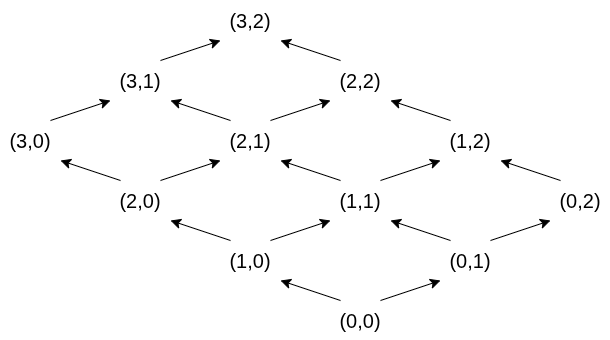
\includegraphics[width=0.5\textwidth]{figures/multi_mva_dependencies2.png}
  \caption{Precedence of exact multi-class MVA intermediate solutions.}
  \label{fig:bg-multiclass-mva-deps}
\end{figure}

\subsubsection*{Approximate Multi-Class MVA}

Similarly to the single-class solution, an approximation for $h$ can be used to maintain an accurate output whilst dramatically reducing space and time requirements, iterating around an estimate. A good approximation for $h$ here is $h_c[Q_{1,k}(\mathbf{N}), \ldots, Q_{c,k}(\mathbf{N})] \equiv \frac{N_c - 1}{N_c} \cdot Q_{c,k}(\mathbf{N}) + \sum_{j \neq c} Q_{j,k}(\mathbf{N})$. Intuitively, the removal of a customer from the network does not affect the placement of other classes, and reduces the queue lengths of its own class proportionally \cite{lazowska84,bard79}.

\begin{algorithm}
\caption{Approximate MVA for multi-class models \cite{lazowska84}}
\begin{spacing}{1.15}
\begin{algorithmic}[1]
\State $Q_{c,k}(\mathbf{N}) \gets \dfrac{N_c}{K}$ for all $c = 1,\ldots,C$ and $k = 1,\ldots,K$
\Repeat
  \State $Q_{c,k}^{\text{old}}(\mathbf{N}) \gets Q_{c,k}(\mathbf{N})$ for all $c,k$
  \For{$c = 1$ to $C$}
    \For{$k = 1$ to $K$}
      \State $A_{c,k}(\mathbf{N}) \gets h_c\bigl[Q_{1,k}(\mathbf{N}),\ldots,Q_{C,k}(\mathbf{N})\bigr]$
    \EndFor
  \EndFor
  \For{$c = 1$ to $C$}
    \For{$k = 1$ to $K$}
      \State $R_{c,k}(\mathbf{N}) \gets \begin{cases}D_{c,k} & \text{(delay centres)} \\ D_{c,k} \bigl(1 + A_{c,k}(\mathbf{N})\bigr) & \text{(queueing centres)}\end{cases}$
    \EndFor
  \EndFor
  \For{$c = 1$ to $C$}
    \State $X_c \gets \dfrac{N_c}{Z_c + \sum_{k=1}^{K} R_{c,k}(\mathbf{N})}$
  \EndFor
  \For{$k = 1$ to $K$}
    \State $Q_{c,k}(\mathbf{N}) \gets \sum_{c=1}^{C} X_c R_{c,k}(\mathbf{N})$
  \EndFor
\Until{$\max_{c,k} \left| Q_{c,k}(\mathbf{N}) - Q_{c,k}^{\text{old}}(\mathbf{N}) \right| \le \varepsilon$}
\end{algorithmic}
\end{spacing}
\end{algorithm}

The time complexity is reduced greatly, to a point where the population of the classes is not considered, $O(C \cdot K)$ per iteration. The space complexity is similarly reduced to $O(C \cdot K)$, as the algorithm only requires maintaining a solution for population $\mathbf{N}$ \cite{lazowska84,bard79}.



\section{Extended Queueing Networks}
\label{sec:bg-extended}

Classical queueing networks and Mean Value Analysis provide efficient solution techniques under product-form assumptions. However, these assumptions are frequently violated in distributed client-server systems. We must therefore assess the limitations of the classical approach and introduce the extensions that motivate Layered Queueing Networks.

\subsection{Assumptions of Product-Form Queueing Networks}
\label{sec:bg-pf-assumptions}

While product-form queueing networks enable efficient computation of performance measures, they rely on the underlying set of Baskett–Chandy–Muntz–Palacios (BCMP) product-form assumptions \cite{franks99, baskett75}:

\begin{itemize}
\item Service centres are of one of these specific types:
\begin{itemize}
\item A single server with a first-come-first-served (FCFS) queueing discipline, where the time a job needs at the server is exponentially distributed. The mean service times for all customers must be identical.
\item A single server with a last-come-first-served (LCFS), service-in-random-order (SIRO) or processor-sharing (PS) discipline. Service time distributions can be general (do not require the memoryless property), and different customers can have different service times.
\item A load-dependent first-come-first-served service centre, where the service rate is dependent on the number of customers at the station only. This subsumes the infinite-server (IS) as the special case $\mu(n) = n\mu$.
\end{itemize}
\item The population of a closed product-form network is fixed.
\item Customer routing is independent of the state of the network.
\end{itemize}

Despite these assumptions seeming restrictive, there are many models that violate them yet produce sufficiently accurate results. However, there are some cases in which product-form queueing networks (PFQNs) cannot be used directly. If these effects were ignored, we could overestimate the throughput of a model as we are not accounting for the time required to acquire the resources \cite{franks99}.

\begin{itemize}
\item \textbf{Systems with simultaneous resource possession.} The service rate at one centre may be dependent on other centres in the network. If a customer holds a resource at one station while waiting at another, for example, multi-programming lock contention or blocking remote procedure calls, the independence assumption breaks.
\item \textbf{Systems with fork–join behaviour.} Forking generates new customers, whilst joining eliminates them, violating the fixed customer population and routing homogeneity assumptions.
\end{itemize}


This is where we consider the \textbf{method of surrogates}, a hierarchical decomposition strategy that accounts for the time needed to acquire simultaneously-held resources by splitting the input model into submodels and iterating between them. Each submodel contains the explicit representation of one of the resources, and a delay centre representing the other. The waiting time for one of the resources is therefore solved and then used as the delay centre input in the other submodel. This process repeats, iterating between submodels until convergence \cite{franks99}.

\subsection{Client–Server Models}
\label{sec:bg-client-server}

To address the limitations of classical queueing networks, we now consider the adaptations that are tailored towards client–server architecture. These approaches all use hierarchical decomposition and the method of surrogates, breaking multi-tier client–server architecture into two-layer systems that are solved iteratively. Whilst the overall approach is similar, they take different implementation forms \cite{franks99}.

\subsubsection*{Stochastic Rendezvous Network Model}

The Stochastic Rendezvous Network (SRVN) model \cite{woodside89} consists of an acyclic graph of clients and servers (referred to as \textit{tasks}), used to model users and both hardware and software components, connected through remote procedure calls (where the clients are blocked until the server responds). The input model is broken down into a set of submodels that each consist of one server, the set of clients that call it, and surrogate delays for the other calls that the clients make. The clients are treated as unique customers, with a population based on the number of instances of the task. The model is then solved by applying one-step MVA to each of the submodels, adjusting the surrogate delays in the other submodels, and iterating until convergence. This allows the modelling of requests with \textit{rendezvous} semantics, in which clients are blocked until servers reply, directly modelling synchronous remote procedure calls and nested service dependencies. Its \textit{task}, \textit{entry}, and \textit{phase} abstractions become LQN's central modelling vocabulary \cite{woodside95,franks99}.

\subsubsection*{Method of Layers}

The Method of Layers (MOL) \cite{rolia95} explores hierarchical decomposition as a solution strategy for client–server systems, partitioning the system into a set of two-level MVA submodels. These are constructed by splitting the input model into a \textit{hardware contention submodel}, containing all tasks as clients and devices as servers, and a \textit{software contention submodel} which, considering only tasks, sorts the model into layers and constructs submodel n by using all tasks on level n as clients and all tasks at level n + 1 as servers. Surrogate delays are also introduced into the software contention submodels after servers that make a call to another task in the input model. Surrogate delays are introduced into the hardware contention submodel, with one for each task. These submodels are solved by iterating from submodel 1 to N − 1 until convergence. These measures are then used as the think and service times in the hardware model, which is solved, and the measures put back into the software submodels. This process repeats until convergence of both. This approach provides a scalable mechanism for analysing systems with synchronous interactions, where the surrogate delays act as approximates for blocking effects without requiring joint state modelling \cite{franks99,rolia95}.

\subsubsection*{Layered Queueing Networks}

The Layered Queueing Network (LQN) \cite{franks99} is the synthesis of the SRVN model and MOL. It inherits SRVN's modelling vocabulary (tasks, entries, phases, synchronous and asynchronous calls) and MOL's solution strategy (hierarchical decomposition into MVA submodels coupled by surrogate delays). LQNs explicitly represent software entities (tasks, entries, activities) with their limited concurrency and synchronous interactions, alongside hardware resources (processors). By structuring the model into layers and representing synchronous calls as rendezvous interactions, LQNs are able to capture blocking, nested service demands and contention effects that arise naturally in multi-tier systems \cite{franks99,franks2009}.

The increased modelling power of LQNs comes at the cost of increased computational and implementation complexity. LQN solvers rely on decomposition techniques, surrogate delays, and approximate variants of MVA combined with fixed-point iteration \cite{lazowska84,franks99}. These techniques have been used in LQNS \cite{franks2009} and in LINE's \texttt{SolverLN} \cite{casale2024}, which support a wide range of modelling constructs such as interlocking, multi-server stations, and complex activity graphs.




\section{Solving Layered Queueing Networks}
\label{ch:lqn}

We now move from the abstract LQN formalism to the algorithmic machinery that solves an LQN model. We introduce the input vocabulary the solvers consume, the decomposition pipeline that turns an LQN into a sequence of product-form submodels, the MVA variants that solve each submodel, further modelling constructs we see later, and the two specific solver implementations against which this project's contribution is measured. We use the Layered Queueing Network Solver (LQNS) \cite{franks2009} as the primary reference implementation for LQN solution techniques, as it is the most widely used and feature-complete realisation of the LQN formalism \cite{franks99}. 


\subsection{LQN modelling basics}
\label{sec:lqn-basics}

LQN's solution apparatus is built on the Stochastic Rendezvous Network model. The inputs to the model are \textbf{tasks}, which represent hardware and software objects (analogous to service centres in flat queueing networks), \textbf{entries}, which define the per-task service demands (analogous to classes), and \textbf{phases} or \textbf{activities}, denoting the different stages of service within entries, allowing situations where remote procedure calls can respond before service is fully completed \cite{franks99,franks2009}.

\subsubsection*{Tasks}

The LQN model classifies tasks in three ways \cite{franks99}:

\begin{itemize}
\item \textbf{Pure clients / reference tasks} are tasks that only send messages. They are used to model input sources such as users or external request streams, as they cycle continuously and never accept calls themselves.
\item \textbf{Pure servers} are tasks that only receive requests, used to model hardware servers such as processors or disks. They are the \textit{leaves} of the call graph.
\item \textbf{Active servers} are tasks that both accept and produce requests. These are typically software processes that handle an incoming call by making nested calls to lower-level tasks.
\end{itemize}

Tasks communicate with each other using the \textbf{send–receive–reply} paradigm, where the client is blocked until it receives a response from the server. Task service times are broken down into phases, with the task responding to the client at the end of phase one and then executing subsequent autonomous phases. Messages are passed to the server on a first-come-first-served basis, but the server can differentiate its actions based on the entry, analogous to classes in conventional queueing networks \cite{franks99}.

Tasks also carry a \textbf{multiplicity} attribute corresponding to the number of concurrent instances of the task. For a reference task this fixes the closed-network population, while for a non-reference task it sets the multi-server capacity at that task's queue, making multiplicity the standard feature for expressing concurrency limits such as thread pools or worker processes.


\subsubsection*{Host and Task layers}

An LQN solver can decompose a model into two types of submodels:

\begin{itemize}
\item A \textbf{host layer} contains one queue station per \textit{processor} and aggregates the demands of all tasks hosted on that processor. The host layer is where physical hardware contention is modelled.
\item A \textbf{task layer} contains the queue for one non-reference task as the server, and its direct callers as clients. The task layer is where \textit{software} contention is modelled.
\end{itemize}


\subsubsection*{Inputs and outputs}

The inputs for the LQN model, based around entries and phases, are the mean total \textbf{execution time} $s_{ep}$ of entry $e$ in phase $p$, the \textbf{squared coefficient of variation} $c^2_{ep}$ for a slice of that execution time, the \textbf{phase type} $pt_{ep}$ (describing how requests are emitted to lower-level servers), the \textbf{external arrival stream} $\lambda_{0e}$ of requests to entry $e$ and the \textbf{mean number of requests} $y_{edp}$ from entry $e$ in phase $p$ to entry $d$. The output we primarily care about is the \textbf{throughput} $\lambda_e$ of entry $e$, however we can also calculate per-entry queue lengths, utilisations, and residence times \cite{franks99}.


\subsection{Solving LQNs}
\label{sec:lqn-solving}

Every LQN solver follows the same four-step pipeline, established in Franks's 1999 thesis \cite{franks99}, formalised by LQNS \cite{franks2009}, and inherited (with paradigm-flexibility extensions) by \texttt{SolverLN} \cite{casale2024}. We describe the pipeline at the algorithmic level here:

\begin{enumerate}
\item \textbf{Decompose the LQN into a sequence of PFQN submodels.} The LQN's tasks and processors are partitioned into a set of host layers and task layers, where each submodel is a separate product-form queueing network whose stations are derived from the LQN's tasks and processors. Different \textit{layering strategies}, introduced below, produce different partitions of the same LQN. The strategy choice is itself an algorithmic parameter that the LQN solvers expose.

\item \textbf{Solve each submodel with an inner MVA kernel.} Once a submodel is produced as a PFQN, it can be handed to an MVA kernel, producing a complete set of \texttt{QN} / \texttt{UN} / \texttt{RN} / \texttt{TN} \textit{outputs}.

\item \textbf{Couple between submodels by updating service and think times.} The outputs of each submodel are then used to update the \textit{inputs} of the other submodels. A task's residence time at its host layer becomes the service time it presents to its callers in the task layer. A caller task's residence time at the callees becomes a contribution to the think time the caller presents to its own host.

\item \textbf{Iterate to a fixed point.} Steps 2 and 3 are repeated until every submodel's outputs converge. The fixed point is the solution to the LQN.
\end{enumerate}

\begin{figure}[h]
  \centering
  \resizebox{\textwidth}{!}{%
    \begin{tikzpicture}[
    >={Stealth[length=2.2mm]},
    node distance=10mm and 8mm,
    every node/.style={font=\small},
    pipestage/.style={
        rectangle, rounded corners=2pt, draw=black!70, line width=0.5pt,
        text width=24mm, align=center, minimum height=11mm, fill=blue!4,
    },
    decision/.style={
        diamond, draw=black!70, line width=0.5pt, aspect=2.6,
        text width=21mm, align=center, inner sep=1pt, fill=orange!8,
    },
    output/.style={
        rectangle, rounded corners=2pt, draw=black!70, line width=0.5pt,
        text width=22mm, align=center, minimum height=9mm, fill=green!6,
    },
    arr/.style={->, line width=0.5pt, draw=black!70},
    looplabel/.style={font=\footnotesize, fill=white, inner sep=1pt},
]
    \node[pipestage] (decompose) {\textbf{Step 1}\\Decompose\\into PFQN\\submodels};
    \node[pipestage, right=of decompose] (solve) {\textbf{Step 2}\\Solve each\\submodel\\(inner MVA)};
    \node[pipestage, right=of solve] (couple) {\textbf{Step 3}\\Couple via\\service/\,think-\\time updates};
    \node[decision, right=of couple] (conv) {\textbf{Step 4}\\Converged?};
    \node[output, right=14mm of conv] (out) {Output\\AvgTable};

    \draw[arr] (decompose) -- (solve);
    \draw[arr] (solve) -- (couple);
    \draw[arr] (couple) -- (conv);
    \draw[arr] (conv) -- node[above, font=\footnotesize] {yes} (out);

    % Outer loop back-arrow: from "no" outcome of decision back to Step 2.
    \draw[arr]
        (conv.south) -- ++(0,-10mm) node[looplabel, pos=0.5, right=1mm] {no}
        -| (solve.south);
\end{tikzpicture}
%
  }
  \caption[The four-step LQN solver pipeline]{
    The standard four-step LQN solver pipeline.
  }
  \label{fig:bg-four-step-pipeline}
\end{figure}

This pipeline gives rise to two distinct kinds of iteration:

\begin{itemize}
\item The \textbf{inner loop} is the iteration \textit{inside} a single MVA variant. This is the recursion over population in exact MVA, or the \texttt{repeat ... until} loop in approximate MVA. The inner loop runs at step 2 of the pipeline above. It produces one submodel's outputs from its inputs.
\item The \textbf{outer loop} is the iteration \textit{over submodels}. This instruments the sweep through every submodel in steps 2 and 3, terminated by step 4's convergence check. One outer iteration is one sweep through every submodel in the ensemble.
\end{itemize}

\begin{figure}[h]
  \centering
  \begin{tikzpicture}[
    >={Stealth[length=2mm]},
    every node/.style={font=\small},
    submodel/.style={
        rectangle, rounded corners=2pt, draw=black!60, line width=0.4pt,
        text width=22mm, align=center, minimum height=6mm, fill=blue!4,
        inner sep=1.2mm,
    },
    submodelfocus/.style={
        rectangle, rounded corners=2pt, draw=black!85, line width=0.8pt,
        text width=22mm, align=center, minimum height=6mm, fill=blue!14,
        inner sep=1.2mm,
    },
    mvanode/.style={
        rectangle, rounded corners=1pt, draw=black!60, line width=0.35pt,
        fill=white, inner sep=0.8mm, font=\footnotesize,
        text width=13mm, align=center, minimum height=4mm,
    },
    arr/.style={->, line width=0.4pt, draw=black!60},
    tinyarr/.style={->, line width=0.35pt, draw=black!55},
    looparr/.style={->, line width=0.5pt, draw=black!75},
    callout/.style={dashed, draw=black!45, line width=0.4pt},
]
    % Row of submodel-solve boxes representing the outer loop's per-iter sweep.
    % S2 is highlighted because it is the submodel being expanded below.
    \node[submodel] (s1) at (0, 0) {Submodel 1\\solve};
    \node[submodelfocus, right=4mm of s1] (s2) {Submodel 2\\solve};
    \node[submodel, right=4mm of s2] (s3) {Submodel 3\\solve};
    \node[right=4mm of s3, font=\small] (sk) {$\cdots$};
    \node[submodel, right=4mm of sk] (sn) {Submodel $E$\\solve};

    \draw[arr] (s1) -- (s2);
    \draw[arr] (s2) -- (s3);
    \draw[arr] (s3) -- (sk);
    \draw[arr] (sk) -- (sn);

    % Outer-loop back-arrow ABOVE the row; bold label sits above the arrow.
    \draw[looparr]
        (sn.north) -- ++(0,6mm) -| (s1.north);
    \node[font=\footnotesize\bfseries, above=0.3mm]
          at ($(s1.north)!0.5!(sn.north)+(0,6mm)$)
          {Outer Loop: coupling fixed-point iteration};

    % Expanded inner-solve view directly below the focused submodel (S2).
    \node[draw=black!80, line width=0.6pt, rounded corners=2pt, fill=orange!6,
          below=16mm of s2, anchor=north, inner sep=2mm,
          label={[font=\footnotesize, yshift=1mm]above:%
                  {\textbf{Inner Solve: exact MVA recursion}}}]
          (innerbox) {%
        \begin{tikzpicture}[baseline]
            \node[mvanode] (mva1) {$Q_k(N{-}1)$};
            \node[mvanode, right=14mm of mva1] (mva2) {$R_k(N)$};
            \node[mvanode, right=14mm of mva2] (mva3) {$X(N)$};
            \node[mvanode, right=14mm of mva3] (mva4) {$Q_k(N)$};
            \draw[tinyarr] (mva1) -- (mva2)
                node[midway, above=1mm, font=\scriptsize, inner sep=0.5pt] {Arrival}
                node[midway, below=0.3mm, font=\scriptsize, inner sep=0.5pt] {Theorem};
            \draw[tinyarr] (mva2) -- (mva3)
                node[midway, above=1mm, font=\scriptsize, inner sep=0.5pt] {Little's}
                node[midway, below=0.3mm, font=\scriptsize, inner sep=0.5pt] {Law};
            \draw[tinyarr] (mva3) -- (mva4)
                node[midway, above=1mm, font=\scriptsize, inner sep=0.5pt] {$Q_k {=} X R_k$};
            % Flat back-arrow; modest depth keeps the inner box compact.
            \draw[tinyarr, looseness=0.5] (mva4.south) to[out=-90,in=-90]
                node[below, font=\scriptsize, inner sep=1pt]
                    {$N \to N{+}1$}
                (mva1.south);
        \end{tikzpicture}%
    };

    % Zoom-callout cone: two dashed lines diverging from S2 down to the inner box.
    \begin{pgfonlayer}{background}
        \draw[callout] (s2.south west) -- (innerbox.north west);
        \draw[callout] (s2.south east) -- (innerbox.north east);
    \end{pgfonlayer}

\end{tikzpicture}

  \caption[Outer fixed-point loop wrapping per-submodel inner MVA solves]{
    The outer fixed-point coupling loop wraps per-submodel inner MVA
    solves.
  }
  \label{fig:bg-outer-vs-inner-loop}
\end{figure}

\subsubsection*{A worked example}
Consider a small LQN with three elements: a reference task \texttt{T1} with closed population $N$ and pure think time $Z_{T1}$, making one synchronous call per cycle to task \texttt{T2}, where \texttt{T2} has host demand $D_{T2}$ on processor \texttt{P1}.

We decompose this into two PFQN submodels, each a closed product-form network sharing \texttt{T1} as its workload source but isolating a different bottleneck:

\begin{itemize}
  \item \textbf{Host submodel P1} models contention at the processor. Its only queueing station is \texttt{P1}, with service demand $D_{T2}$. \texttt{T1} appears as an IS-delay client whose think time considers everything \texttt{T1} does when not at \texttt{P1}.
  \item \textbf{Task submodel T2} models contention at the task. Its only queueing station is \texttt{T2}'s service queue, and \texttt{T1} is the client. \texttt{T2}'s service time here is its residence time at \texttt{P1}, a value supplied by the host submodel.
\end{itemize}

The two submodels are coupled by \texttt{T2}'s residence time at \texttt{P1} flowing forward into \texttt{Task Submodel T2}, and \texttt{T1}'s response time at \texttt{T2} flows backwards into \texttt{Host Submodel P1}. One \textit{outer iteration} is four steps:

\begin{enumerate}
  \item \textbf{Solve Host Submodel \texttt{P1}} with MVA, returning $R_{T2}^{P1}$ (pure demand plus some queueing).
  \item \textbf{Push forward}: set \texttt{T2}'s service time in \texttt{Task Submodel T2} to $R_{T2}^{P1}$.
  \item \textbf{Solve Task Submodel \texttt{T2}} with MVA, returning $R_{T1}^{T2}$ (one full \texttt{T1}$\to$\texttt{T2} call). 
  \item \textbf{Push back}: set \texttt{T1}'s think time in \texttt{Host Submodel P1} to $Z_{T1} + R_{T1}^{T2}$.
\end{enumerate}

Convergence is declared when those scalars stop moving between successive sweeps. 

\begin{figure}[h]
  \centering
  \begin{subfigure}[c]{0.26\textwidth}
    \centering
    \begin{tikzpicture}[
    >={Stealth[length=2.2mm]},
    every node/.style={font=\small},
    task/.style={
        rectangle, rounded corners=2pt, draw=black!70, line width=0.5pt,
        text width=14mm, align=center, minimum height=8mm, fill=blue!4,
    },
    refnode/.style={task, fill=green!8},
    proc/.style={
        ellipse, draw=black!70, line width=0.5pt, inner sep=1pt,
        minimum width=15mm, minimum height=7mm, fill=orange!8,
    },
    callarr/.style={->, line width=0.5pt, draw=black!70},
    hostarr/.style={-, line width=0.5pt, draw=black!60, dashed},
    elabel/.style={font=\footnotesize, color=black!75},
]
    \node[refnode] (T1) at (0, 0) {T1\\(REF)};
    \node[task, below=10mm of T1] (T2) {T2};
    \node[proc, below=10mm of T2] (P1) {P1};

    \draw[callarr] (T1) -- node[elabel, right=1mm] {sync call} (T2);
    \draw[hostarr] (T2) -- node[elabel, right=1mm] {hosted on} (P1);
\end{tikzpicture}

    \caption{The original LQN.}
    \label{fig:bg-two-submodel-lqn}
  \end{subfigure}%
  \hspace{0.03\textwidth}%
  \begin{subfigure}[c]{0.70\textwidth}
    \centering
    \resizebox{\textwidth}{!}{\begin{tikzpicture}[
    >={Stealth[length=2.5mm]},
    every node/.style={font=\small},
    submodel/.style={
        rectangle, rounded corners=3pt, draw=black!70, line width=0.6pt,
        align=center, fill=blue!3, inner sep=3mm,
    },
    queue/.style={
        rectangle, draw=black!70, fill=orange!12,
        minimum width=12mm, minimum height=9mm,
        font=\scriptsize, align=center,
    },
    delay/.style={
        ellipse, draw=black!70, fill=green!12,
        inner sep=1pt, minimum width=13mm, minimum height=9mm,
        font=\scriptsize, align=center,
    },
    flow/.style={->, line width=0.4pt, draw=black!60},
    couple/.style={->, line width=0.9pt, draw=red!70!black},
    pushbadge/.style={
        circle, draw=red!75!black, fill=red!8,
        line width=0.5pt, inner sep=0pt,
        minimum size=4.5mm, font=\footnotesize\bfseries,
        text=red!75!black,
    },
    solvebadge/.style={
        circle, draw=black!70, fill=yellow!22,
        line width=0.5pt, inner sep=0pt,
        minimum size=4.5mm, font=\footnotesize\bfseries,
        text=black!85,
    },
    sublabel/.style={font=\footnotesize, color=black!85, align=center},
    boxtitle/.style={font=\small\bfseries},
]

    %---- HOST submodel (left) ----
    \node[submodel] (host) {%
        \begin{tikzpicture}[baseline]
            \node[delay] (t1h) {T1\\(IS-delay)};
            \node[queue, right=8mm of t1h] (p1) {P1\\(queue)};
            \draw[flow] (t1h.east) -- (p1.west);
        \end{tikzpicture}%
    };
    \node[boxtitle, above=0.5mm of host] {Host Submodel P1};
    \node[solvebadge] at ([xshift=4mm,yshift=-4mm]host.north west) {1};

    %---- TASK submodel (right) ----
    \node[submodel, right=30mm of host] (task) {%
        \begin{tikzpicture}[baseline]
            \node[delay] (t1t) {T1\\(client)};
            \node[queue, right=8mm of t1t] (t2) {T2\\(queue)};
            \draw[flow] (t1t.east) -- (t2.west);
        \end{tikzpicture}%
    };
    \node[boxtitle, above=0.5mm of task] {Task Submodel T2};
    \node[solvebadge] at ([xshift=4mm,yshift=-4mm]task.north west) {3};

    %---- Step 2: forward push (arc over the top, host -> task) ----
    \draw[couple] (host.north east) to[out=45, in=135]
        coordinate[midway] (topmid)
        (task.north west);
    \node[pushbadge] (b2) at (topmid) {2};
    \node[sublabel, above=0.5mm of b2, align=center]
        {push $R_{T2}^{P1}$\\$\to$ T2's service time};

    %---- Step 4: back push (arc under the bottom, task -> host) ----
    \draw[couple] (task.south west) to[out=-135, in=-45]
        coordinate[midway] (botmid)
        (host.south east);
    \node[pushbadge] (b4) at (botmid) {4};
    \node[sublabel, below=0.5mm of b4, align=center]
        {push $R_{T1}^{T2}$\\$\to$ T1's think time};

\end{tikzpicture}
}
    \caption{The two-submodel coupling loop produced by
      \texttt{SolverLN.buildLayers}.}
    \label{fig:bg-two-submodel-coupling}
  \end{subfigure}
  \caption[Two-submodel ensemble decomposition and coupling for the worked example]{
    Decomposition and outer-loop coupling for the worked example.
  }
  \label{fig:bg-two-submodel-example}
\end{figure}

\subsection{MVA variants} 
\label{sec:lqn-mva-variants}

Solving each submodel is parametric in which MVA variant we choose. No single variant is uniformly best: submodels differ in size, in whether stations have population-dependent service rates, and in how tight an accuracy/cost trade-off the caller can tolerate. We cover the MVA variants that arise in practice:

\textbf{Exact MVA} refers to the Reiser–Lavenberg recursion \cite{reiser80} from Section~\ref{sec:bg-mva}, giving the exact solution for any closed product-form network. Multi-class cost is exponential in the number of classes, so it is competitive only when the lattice size, the population combinations that build the solution, $\texttt{prodN} = \prod_c (N_c + 1)$ is small.

\textbf{Load-Dependent MVA (LD-MVA)} \cite{reiser81} generalises exact MVA to stations with population-dependent service rates $\mu_k(j)$, conditioning the recursion on a queue-length distribution table $\pi(k \mid n)$ \cite{lazowska84}. It is the standard kernel when a submodel contains a multi-server task whose rate must be modelled exactly.

\textbf{Bard–Schweitzer Approximate MVA (AMVA)} \cite{bard79} replaces the exact arrival-instant relation with $A_k(N) \approx \frac{N - 1}{N} Q_k(N)$, seen in Section~\ref{sec:bg-mva}, yielding a cheap $O(C \cdot K)$-per-iteration fixed point on residence times.

\textbf{Linearizer} \cite{chandy82} refines Bard–Schweitzer with a second-order correction on the arrival-instant queue length, improving accuracy at moderate populations \cite{zahorjan88}.

\textbf{Seidmann's transform} \cite{seidmann87} folds a $c$-server station with demand $L$ into a single-server station with demand $L/c$ and a $Z$-shift of $L(c-1)/c$, with total queue length reconstructed via $Q_{\text{total}} = Q_{\text{BS}} + X \cdot L(c-1)/c$. It was extended to LQN solvers by Rolia \cite{rolia92}, to keep the cheap single-server MVA kernels applicable when tasks and processors have multiplicity greater than one.

\subsection{Further solver constructs}
\label{sec:lqn-other-machinery}

Mature solvers layer additional modelling constructs on top of the pipeline above, and are ideas we revisit throughout the contribution and evaluation chapters.

\textbf{Activity graphs.} Richer LQN models can be described by a directed precedence graph, whose nodes are activities and whose edges are typed. The edges can be a \textbf{sequence}, running activities in order, an \textbf{OR-fork}, branching probabilistically, an \textbf{AND-fork}, spawning parallel branches that an \textbf{AND-join} later synchronises, or a \textbf{loop}, repeating a body. A \textbf{reply} marks the point at which the caller's phase-1 synchronous wait ends, so any work after the reply is the autonomous phase-2 body that the processor still executes but the caller does not perceive. Because an AND-join completes only when its slowest branch does, the caller-perceived join delay is the \textit{expected maximum} of the branch times. For exponentially distributed branches, this reduces to the inclusion-exclusion sum, though in practice solvers approximate it \cite{franks99}. Activity graphs are what let an entry express conditional, parallel and iterative control flow rather than a single straight-line demand.

\textbf{Under-relaxation.} The outer fixed-point iteration is not guaranteed to converge monotonically and can instead oscillate, with a quantity overshooting on one sweep and undershooting on the next. Solvers mitigate this by moving a coupled input only a fraction $\alpha$ of the way to its newly computed value, $x \leftarrow (1-\alpha)\,x_{\text{old}} + \alpha\,x_{\text{new}}$, rather than overwriting it outright.

\textbf{Interlocking.} When a server is reached along several call paths that share a common ancestor task, the requests along those paths are not independent as a customer busy in one path cannot simultaneously be in any of the others. Treating the paths as independent would therefore overestimate the contention the server sees, inflating throughput values. Interlocking is the correction LQNS applies, discounting a server's queueing by the fraction of its load that originates from a shared caller \cite{franks99,franks2009}. Computing it requires walking the call graph to find the interlocked paths and their loads.

\subsection{The Layered Queueing Network Solver (\texttt{LQNS})}
\label{sec:lqn-lqns-v5}

LQNS is the mature canonical reference implementation of an LQN solver, described formally in Franks et al. (TSE 2009) \cite{franks2009} and the LQNS user manual \cite{franks2022manual}. Its solution follows the four-step pipeline of Section~\ref{sec:lqn-solving} with the following specific choices.

\textbf{Step 1: Decomposition into PFQN submodels.} LQNS supports four layering strategies, each producing a different submodel partition of the same LQN:

\begin{itemize}
\item \textbf{Batched layering} is LQNS's default strategy. Submodel $l$ contains every task and processor at nesting level $l + 1$ as servers, with clients being any task that calls one of those servers \cite{franks99}.
\end{itemize}

\begin{itemize}
\item \textbf{Strict layering} is the Method of Layers strategy \cite{rolia95}. Software submodels are built top-down level by level, with all tasks at level $L$ as clients and all tasks at level $l + 1$ as servers \cite{franks99}. The hardware submodel has all tasks as clients and all devices as servers. Strict layering produces fewer but larger submodels than Batched.
\end{itemize}

\begin{itemize}
\item \textbf{Loose layering} is the strategy of the SRVN solver \cite{woodside89}. Each serving task or processor becomes its own submodel, with its callers as clients \cite{franks99}. Loose layering produces the largest number of submodels but the simplest individual submodels, many of which are one-class, single-server PFQNs.
\end{itemize}

\begin{itemize}
\item \textbf{Squashed layering} collapses the entire LQN into a single submodel, with pure clients appearing as clients, pure servers as servers, and active servers appearing in both \cite{franks99}. Squashed layering is rarely used in practice but is a useful reference point when comparing layering strategies, representing the extreme of having no decomposition.
\end{itemize}

\textbf{Step 2: Inner MVA kernel.} LQNS's default inner kernel is the Linearizer \cite{chandy82}, with Bard–Schweitzer as a fallback.

\textbf{Step 3: Coupling.} LQNS couples between submodels via \textbf{surrogate delays}, the central coupling mechanism of MOL \cite{rolia95}. A delay centre is inserted into each submodel to represent the time customers spend at servers in other submodels they call. The surrogate delay value is updated between iterations from the residence time of the callee submodel.

\textbf{Step 4: Iteration.} LQNS iterates submodels in a top-down then bottom-up \textit{elevator} order, terminating when a per-station residence time delta falls below tolerance. This allows both think times to be propagated down and wait times to be propagated up equally, providing good estimates early on \cite{franks99}.

\subsection{\texttt{SolverLN}: LINE's layered solver}
\label{sec:lqn-solverln}

This project's \textit{primary} comparator is \texttt{SolverLN}, the LINE codebase's layered solver, described formally in Casale, Gao, Niu and Zhu (2024) \cite{casale2024}. LINE is the open-source queueing analysis framework motivated by the observation that practitioner tooling has historically concentrated on just two paradigms, discrete-event simulation and approximate mean-value analysis, despite deeper stochastic-methods literature \cite{casale2020wsc}. Its design response pairs a single modelling language with interoperable solver backends (MVA, NC, MAM, FLUID, CTMC, LDES, plus external dispatch to JMT and LQNS), and \texttt{SolverLN} inherits this multi-paradigm reach as per-layer solver dispatch, where LQNS commits to approximate MVA at every submodel \cite{casale2024}.

Of the per-layer paradigms \texttt{SolverLN} can dispatch, this project engages with the MVA path specifically. \texttt{SolverLN} inherits significant machinery from LQNS by direct porting, the two solvers therefore belong to the same tool family. This project's bottom-up methodology is a deliberate response to this propagation pattern. Building from a base case rather than carrying inherited machinery forward unexamined allows us to investigate the impact of each component. For this project, \texttt{SolverLN} is the primary comparator because we make the decision to consume the same submodel ensemble produced by \texttt{SolverLN.buildLayers}, meaning iteration counts on both can be compared on like terms.

\subsection{Iteration economy in prior LQN solvers}
\label{sec:lqn-related-work}

This section explores LQN solver literature on iteration economy and solver simplification. The two papers we explore are Casale et al.'s 2024 TOMACS paper introducing \texttt{SolverLN} \cite{casale2024} and Franks and Li's 2012 ICPE paper on inner-loop reduction inside LQNS \cite{franksli2012}. Clearly, however, the outer-loop of these solvers have received very little analysis, and its individual pieces of machinery have not been evaluated against the correctness-efficiency trade-off that removing them exposes. Therefore, we will discuss what is achieved in each of these papers, what is not done, and how it relates to our project.

\subsubsection*{Casale et al.\ (2024): The LN meta-solver}

Casale, Gao, Niu and Zhu's \textit{LN: A Flexible Algorithmic Framework for Layered Queueing Network Analysis} \cite{casale2024} contributes a per-layer paradigm dispatch. Each submodel can be solved through any of LINE's methods (normalising-constant (NC) analysis, MVA, matrix-analytic methods, fluid mean-field approximation, continuous-time Markov chain analysis and discrete-event simulators), however the Table 2 heuristic dispatch narrows the scope to NC and MVA only. More specifically, selection criteria route single-class, single-server, and small-population models to NC and routes multiclass multiserver, high-or-medium-population, and non-product-form models to MVA. The evaluation in Section 6.1 is performed on a random 30-model LQN corpus, where the heuristic chose NC approximately 90\% of the time. The paper also introduces a non-iterative MVA approximation for networks containing just one delay node and $m$ identical queueing stations, known as homogeneous closed networks, in Section 5.4, providing a significantly more accurate approximation than the asymptotic bounds typically used to initialise LQN submodels.

However, despite the paper describing how the outer loop of the solver behaves, it does not analyse it to the same level as the inner loop. The convergence test, described in Subsection 3.3.4, depends on the largest per-class change in mean queue length between iterations, $\Delta_{i+1,l} = \max_r |Q_r^{(i)} - Q_r^{(i+1)}| / N_r$, and is summed across submodels, $\Delta_{i+1} = \sum_l \Delta_{i+1,l}$, with a moving window applied to residence times and throughputs when convergence is not reached within a maximum number of iterations. This is implemented in LINE with an \texttt{iter\_min} floor, a sliding-window weighted average over  \texttt{QN}/\texttt{UN}/\texttt{RN}/\texttt{TN}, multi-iteration sub-tolerance and a verification pass that the paper does not describe. Furthermore, the elevator iteration pattern over submodels is inherited directly from Franks's thesis \cite{franks99}.

Our project takes this, retaining \texttt{SolverLN}'s submodel decomposition, asking which pieces of the outer-loop structure are necessary for closed LQN models. We also look into isolating specific \texttt{SolverLN} features, and the effect that removal has on both precision and efficiency. \texttt{SolverLN}'s own design already treats some iterative machinery as optional on the homogeneous submodel, therefore we question whether the outer-loop scaffolding allows the same.

\subsubsection*{Franks and Li (2012): One-Step MVA}

Franks and Li's \textit{Efficiency Improvements for Solving Layered Queueing Networks} \cite{franksli2012} is the primary iteration-economy paper in the LQN space. The paper takes the three loops seen in LQNS (an outer fixed-point iteration over submodels, Linearizer's main two-pass loop, and Bard--Schweitzer's \texttt{repeat \dots until}) and constructs two new variants. One-Step Linearizer (OSL) drops Linearizer's outer two-iteration loop and skips the redundant \texttt{core(N)} invocation that begins each subsequent call, instead warm-starting from the previous submodel's solution. One-Step MVA (OSM) further removes Bard-Schweitzer's \texttt{repeat \dots until} entirely, letting the outer LQNS loop take its place. The evaluation is on the thirteen-layer Bookstore model from Israr, Woodside and Franks (2007) \cite{israr2007}, with four solver configurations (Linearizer, OSL, Bard-Schweitzer, OSM) crossed with five submodel-layering strategies (Batched, Hardware-Software, MOL, Squashed, SRVN). Performance was evaluated on calls to \texttt{wait()}, representing one step of MVA. Under MOL layering, Linearizer made $87{,}852 \times 10^4$ calls while OSM only required $7 \times 10^4$, a reduction of approximately $12{,}500\times$. Throughput results agreed to four decimal digits across the grid, whilst run time fell from 01:47 to 00:06. The paper notes however, that the number of outer iterations sometimes increased, confirming the paper's own hypothesis that work formerly done by inner-loop convergence is absorbed into additional outer-loop sweeps.

Once again, however, this paper's reductions focus on the inner AMVA loop rather than the outer loop. The motivating observation in the Conclusions section, \textit{``Much of the work obtaining `accurate' solutions during early iterations of the outer-most loop is wasted because the parameters for a given submodel are going to change anyway due to solutions to other submodels''} \cite{franksli2012}, is used to justify collapsing the inner loop, on the basis that the outer fixed-point iteration will invalidate any over-precise submodel solution. The outer loop itself, however, is left unchanged.

We therefore look to see if there is a similar reduction we can achieve on the outer loop from a stripped back version of the solver. Whilst their reduction asks whether the inner AMVA loop's full convergence is necessary given the outer loop's re-run, we ask whether specific outer-loop machineries are necessary, given the structure of submodel coupling.
